\documentclass{article}

    %the math packages
    \usepackage{amsmath,amsfonts,amssymb,amsthm}
    \theoremstyle{plain}
    \newtheorem{thm}{Theorem}[section]
    \newtheorem{lem}[thm]{Lemma}
    \newtheorem{prop}[thm]{Proposition}
    \newtheorem*{cor}{Corollary}
    
    \theoremstyle{definition}
    \newtheorem{defn}{Definition}[section]
    \newtheorem{conj}{Conjecture}[section]
    \newtheorem{exmp}{Example}[section]
    
    \theoremstyle{remark}
    \newtheorem*{rem}{Remark}
    \newtheorem*{note}{Note}
    
    \usepackage{mathtools}
    \usepackage{optidef}
    %add new math packages here
    
    %--------------------------
    
    
    %the algorithm packages
    \usepackage{algorithm}
    \usepackage{algorithmicx}
    \usepackage{algpseudocode}
    \algrenewcommand\algorithmicrequire{\textbf{Input:}}
    \algrenewcommand\algorithmicensure{\textbf{Output:}}
    %add new algorithm packages here
    
    %-------------------------------
    
    \usepackage{graphicx}
    \usepackage{tikz}
    \usepackage{subfigure}

    \usepackage{natbib}
    
    % In case you need to adjust margins:
    \topmargin=-0.45in      %
    \evensidemargin=0in     %
    \oddsidemargin=0in      %
    \textwidth=6.5in        %
    \textheight=9.0in       %
    \headsep=0.25in         %
    
    %newcommand for the format of the homework
    \newcommand{\Answer}{\ \\\textbf{Answer:} }
    \newcommand{\Acknowledgement}[1]{\ \\{\bf Acknowledgement:} #1}
    
    \newcommand\numberthis{\addtocounter{equation}{1}\tag{\theequation}}
    %end the newcommand for this part
    
    %new command for the partial derivatives
    \newcommand{\pd}[2]{\frac{\partial #1}{\partial #2}}
    \newcommand{\spd}[3]{\frac{\partial^2 #1}{\partial #2 \partial #3}}
    \newcommand{\grad}[1]{\nabla #1}
    \newcommand{\curl}[1]{\nabla \times #1}
    \newcommand{\dive}[1]{\nabla \cdot #1}
    %end the new command for this part
    
    \title{\bf\huge Network Science Project Report}
    \author{Haoyu Zhao,2016012390}
    \date{}
    
    \begin{document}
    \maketitle

    \section{Introduction}
    \subsection{Introduction to the Problem}
    In this project, we study a problem that is related to both online decision problem, or more specificly, the multi-armed bandit, and the information synchronization problem. The problem is useful in the real life, especially in the distrubuted computing and system field. For example, the distributed file storage system may need to synchronize the file data through the communication network, and in a multi-agent setting, each agent needs to transfer the information to coordinate the action. However, usually we do not know the cost of connecting between 2 nodes in a communication network before we actually choose to connect, and moreover, we may not know the distrubution of that cost, so we need to make decision and change our estimation online.

    \subsection{Basic Settings and Problem Formulation}
    In this section, we state our problem and the basic settings formally. Given a graph $G(V,E)$ as a conmunication network, and each node $v\in V$ has it's own information $I_v$. Then we want to synchronize the information in the network, i.e. each node know the information of all other nodes. Each time the information goes from $u$ to $v$, $u$ can transfer all the information to $v$.\\

    Our problem is the online repeated version of this information synchronization problem. We know the graph topology $G(V,E)$, but we do not know the weight of each edge. There is a random variable $X_e$ as the weight of edge $e$ and we do not know the distribution of $X_e$. Assume that we want to synchronize the information in many rounds, and in each round, the weight of each edge will not change. If we choose edge $e$ in round $t$, then we can know the value of $X_e$ in round $t$.\\

    In this project, we focus on 2 different aspect of the problem. The first aspect is that we want to minimize the cost of the information synchronization process. Under this setting, the weight of each edge $e$ in round $t$ is the cost of using this edge in round $t$, which is not affected by the number of times we use this edge to transfer the information in this round and by the amount of information we transfer during one usage of the edge. Formally, let $X_{e,t}$ denote the cost of edge $e$ in round $t$, what we want to do is to select $S_t$ in each round $t$, such that the expectation of the total cost
    \[\mathbb E\sum_{e\in S_T}X_{e,t},\]
    with the constraint that the information synchronization can be completed successfully.\\

    The other aspect is that we want to minimize the time of the information synchronization process. Under this setting, the weight of each edge $e$ in round $t$ is the time that information transfer from $1$ endpoint of that edge to another. We also assume that the in each round, the time needed to transfer the information does not change. Formally, let $X_{e,t}$ denote the time needed by edge $e$ in round $t$, what we want to do is to choose a sequence of edges that synchronize the information as fast as possible(allow transfer the information parallel on different edges).

    \subsection{Hardness of the Problem}
    \subsubsection{Exploration vs. Exploitation}
    How to balance the exploration and exploitation is a general problem in the online learning, and especially the multi-armed bandit field. To get more accurate estimation of each random variable, we should observe that random variable for as more time as possible. However, if we choose the random variable that is `bad' ,i.e. it may cost a lot to choose that variable, we should not observe that random variable. So there is a seemingly contradiction between the exploration and exploitation, and we should balance these 2 aspect.

    \subsubsection{Exponential Number of Feasible Action}
    Given a graph with $n$ edges, we can have $2^n$ number of possible actions, although some of them violate the constraints. Then just consider the spanning tree of a complete graph, the number of spanning trees is also exponential compared with the number of edges. So given the time horizon of our repeated online information synchronization problem, we may not try each feasible action once.

    \subsubsection{Different Kinds of Measurements}
    Different kinds of measurements of the information synchronization also lead to a challenge of the problem. Because when we want to optimize the objective function under different measurements, such as cost, time or a combination of them, we will often lead to different algorithm and models. So it may hard to combine different kind of model under a general framework and get theoretical guarantee of the algorithm performance.

    \subsection{Related Works}

    \section{Methods to Solve the Problem}
    \subsection{General Methods}
    To tackle the problem of the unknown distribution of the edges, we apply the framework in multi-arm bandit. However, in the network information syncronization setting, the number of possible result will be exponentially large with respect to the number of nodes. Fortunately, \cite{chen2013combinatorial} gave a framework of combinatorial multi-armed bandit to deal with the problem of exponentially number of `arms'. We apply the framework, and the algorithm in that framework, and combine it with the network information synchronization problem. The algorithm is shown in \textbf{Algorithm \ref{cucb}}

    \begin{algorithm}
        \caption{Algorithm to solve the online information syncronization problem}
        \label{cucb}
        \begin{algorithmic}[1]
        \Require The graph structure(without weight) $G(V,E)$, and the algorithm $\mathcal A$ we want to run online.
        \Ensure The action of each round
        \Procedure{Alg}{$G(V,E),\mathcal A$}
            \State $\hat \mu_i \leftarrow$ the empirical expectation of edge $i$.
            \State $T_i \leftarrow$ the number of time the edge $i$ is used.
            \State Every time we use an edge $i$, we will update the empirical expectation $\hat \mu_i$ and the counter $T_i$.
            \For{$t = 1,2,\dots,|E|$}
                \State Play an instance from all possible instances which contains the egde $i$.
            \EndFor
            \For{$t=|E|+1,\dots$}
                \State $\bar\mu_i \leftarrow \hat\mu_i - \sqrt{\frac{3\ln t}{2T_i}}$.
                \State Play an instance which minimize the result of algorithm $\mathcal A$ when each edge has weight $\bar\mu_i$.
            \EndFor
        \EndProcedure
        \end{algorithmic}
    \end{algorithm}

    \subsection{Minimize the Total Cost}
    In this section, we consider the setting when we want to minimize the cost of information synchronization in the network. Now suppose that the random variable $X_i$ on edge $i$ represents the cost of select edge $i$. In this setting, we just consider the total cost but not consider the other measurements. To make the model simple, we assume that if we choose an edge, we will pay for the cost of setting up the connection, and the cost is independent of how much information we transfer or how many times we transfer the information.\\
    
    This setting is reasonable in many real life cases when the information synchronization does not have constraints on time but the cost of communication is large, especially when the information synchronization does not happen so often and the cost of synchronization is high. We have the following simple theorem under this setting, and we assume that the random variables that represent the cost on each edge are positive.\\

    \begin{thm}\label{min-spanning-tree}
        Under the senerio of minimizing the total cost while synchronizing the information, the edges that are chosen by the optimal strategy will form a spanning tree.
    \end{thm}
    \begin{proof}
        This theorem is really simple. First because we want to synchronize the information for all nodes, the chosen edges will let all of the nodes to be connected. Then because all of the edges have positive cost, then if there is a cycle it must be non-optimal. So the optimal strategy will choose a spanning tree of the graph.
    \end{proof}

    Now it is obvious that the best strategy tries to find the minimum expectation cost spanning tree, which is the spanning tree that minimize the total cost in the long term. We have the following algorithm, see \textbf{Algorithm \ref{cucbmintree}}, which follows the framework \textbf{Algorithm \ref{cucb}}.

    \begin{algorithm}
        \caption{Algorithm to solve the problem under the min cost setting}
        \label{cucbmintree}
        \begin{algorithmic}[1]
        \Require The graph structure(without weight) $G(V,E)$.
        \Ensure The action of each round, where the edge selected in each round forms a spanning tree of all the nodes and then the algorithm tries to minimize the long term total cost of the spanning tree.
        \Procedure{Alg}{$G(V,E)$}
            \State $\hat \mu_i \leftarrow$ the empirical expectation of edge $i$.
            \State $T_i \leftarrow$ the number of time the edge $i$ is used.
            \State Every time we use an edge $i$, we will update the empirical expectation $\hat \mu_i$ and the counter $T_i$.
            \For{$t = 1,2,\dots,|E|$}
                \State Find an arbitrary spanning tree that contains edge $t$.
            \EndFor
            \For{$t=|E|+1,\dots$}
                \State $\bar\mu_i \leftarrow \hat\mu_i - \sqrt{\frac{3\ln t}{2T_i}}$.
                \State Find the minimum spanning tree with $\bar\mu_i$ as the weight on edge $i$.
            \EndFor
        \EndProcedure
        \end{algorithmic}
    \end{algorithm}

    Now the only problem is how to find the minimum spanning tree of a graph. The problem is simple and we can use Kruskal's algorithm. Then given a spanning tree of the graph, we can transfer the information through the edges of the tree and we can synchronize the infromation.

    \subsection{Minimize the Maximum Time}
    In this subsection, we consider the case when we want to minimize the time when we synchronize all the information. Here we assume that the weight of each edge $e = (u,v)$ represent the time that information goes from $u$ to $v$ or $v$ to $u$.

    \subsubsection{A very simple case}
    Now we start from a simple case of our problem, we add an assumption about our problem.\\
    
    \textbf{Assumption:} The cost of each edge is a constant, and we know the constant.\\
    
    Under this setting, the fastest way to complete the information synchronization is that $\forall u,v\in V$, $u$ send the information to $v$ through the shortest path between $u,v$ and $v$ send the information to $u$ along the shortest path from $v$ to $u$. However, finding the union of the shortest path of all pair of points usually has $O(n^2)$ edges, and it is very wasting if every edge just transfer little information.\\

    Here we use another method to transfer the information, which is an approxiamtion of the theoretical optimal solution, and use the minimum possible number of edges. We need the following definition.

    \begin{defn}\label{center}
        (Center) Given a graph $G(V,E)$, we call a vertex $v\in V$ the center of graph $G$, such that
        \[v = \arg\min_{u\in V}\{\max_{u'\in V}\text{dist}(u,u')\},\]
        where $\text{dist}(u,u')$ denotes the shortest distance from $u$ to $u'$.
    \end{defn}

    Now given $G(V,E)$, denote $v\in V$ as the center of graph $G$, then denote $T$ as the shortest path tree rooted at $v$. The shortest path tree only has $|V|-1$ edges so it is really saving when we no not have so much cost. Moreover, we have the following theorem which shows that given the center and the shortest path tree rooted at the center, the strategy is not so bad.

    \begin{thm}
        If $v\in V$ is the center of graph $G(V,E)$ and $T$ is the shortest path tree of $G$ rooted at $v$, then consider the following strategy, all of the node transfer it's own information to $v$ through tree $T$, and after collecting all the information, the node $v$ transfer all of the information to each nodes. Then this strategy is a $2$ approximation with respect to the time, i.e. it cost at most twice the time of the optimal strategy.
    \end{thm}

    \begin{proof}
        The proof is really simple. Denote $d = \min_{u\in V}\{\max_{u'\in V}\text{dist}(u,u')\}$, which is the maximum distance from the center $v$ to any other nodes. Then denote $d' = \max_{u,u'}\text{dist}(u,u')$, there $\text{dist}$ denote the shortest path length between $u,u'$. Then we know that $d$ is the time required by our strategy, and $d'$ is the time required by the optimal strategy. Then we have
        \[d' = \text{dist}(u,u') \le \text{dist}(u,v) + \text{dist}(v,u') \le d + d = 2d.\]
    \end{proof}

    Now given the theorem, we know that if we can find the center of the graph and then figure out the shortest path tree rooted at the center, then the solution is a good approximation of the optimal solution, and the number of edges is minimized.\\

    Now the only problem is how to find the center and the shortest path tree. First we call the `All Pair Shortest Path' algorithm to find the shortest distance between every $2$ nodes, and we denote the distance matrix $D$, such that $d_{ij} = \text{dist}(v_i,v_j)$. Then we find $c = \arg\min_{i}\max_j d_{ij}$, then $c$ is the center of the graph. At last we call the shortest path algorithm to find the shortest path tree rooted at $c$.\\

    We know that `All Pair Shortest Path' problem can be solved in $O(n^3)$ by the Floyd algorithm, and the shortest path tree can be found by Dijkstra algorithm, and the total running time is $O(n^3)$.

    \subsubsection{A not so simple case}
    Now we consider a not so simple case, which we have the assumption that the each random variable is a constant but we do not know the constant. Then our solution is to call the algorithm framework (\textbf{Algorithm \ref{cucb}}), and turned it into the online version, see \textbf{Algorithm \ref{cucbcentertree}}.

    \begin{algorithm}
        \caption{Algorithm to solve the problem under the min time setting}
        \label{cucbcentertree}
        \begin{algorithmic}[1]
        \Require The graph structure(without weight) $G(V,E)$.
        \Ensure The action of each round, where the edge selected in each round forms a spanning tree of all the nodes and then the algorithm tries to find the minimize the information transfer time in the long term.
        \Procedure{Alg}{$G(V,E)$}
            \State $\hat \mu_i \leftarrow$ the empirical expectation of edge $i$.
            \State $T_i \leftarrow$ the number of time the edge $i$ is used.
            \State Every time we use an edge $i$, we will update the empirical expectation $\hat \mu_i$ and the counter $T_i$.
            \For{$t = 1,2,\dots,|E|$}
                \State Find an arbitrary spanning tree that contains edge $t$.
            \EndFor
            \For{$t=|E|+1,\dots$}
                \State $\bar\mu_i \leftarrow \hat\mu_i - \sqrt{\frac{3\ln t}{2T_i}}$.
                \State Find the center of the graph $G$ and the corresponding shortest path tree rooted at the center with $\bar\mu_i$ as the weight on edge $i$.
            \EndFor
        \EndProcedure
        \end{algorithmic}
    \end{algorithm}


    \subsubsection{Another not so simple case}
    Now we consider the case that the distribution of each random variable on the edge is known. Similar as the previous discussion, we also want to find a `center' of the graph and a spanning tree rooted at the center, such that the spanning tree minimize the largest distance from the center we choose. Formally, we want to find a spanning tree $T$ rooted at $v$ such that
    \[\mathbb E[\max_{u,T}\text{dist}(v,u)],\]
    is minimized, where the distance function $\text{dist}$ denote the shortest path from $v$ to $u$ on the tree $T$.\\

    Note that computing the exact spanning tree that minimize the objective function may be difficult, and we try an approximate solution. We compute the mean weight of each edge and we find the center and the corresponding shortest path tree rooted at the center with respect to the mean of each weight. Our solution is approximate because of the following fact of the objective functions,
    \[\mathbb E[\max_{u,T}\text{dist}(v,u)] \ge \max_{u,T}\mathbb E[\text{dist}(v,u)],\]
    since the max function is convex. Then the algorithm is the same as the most simple case, given the mean of each edge.

    \subsubsection{The general case}
    Then in the general case, we do not know the distribution of the random variables. We also use the approximate solution as shown in the previous case. Then combined with the online settings, we can thus reuse the algorithm when the random variables are constants, see \textbf{Algorithm \ref{cucbcentertree}}.

    \section{Simulation}
    \subsection{Minimize the Total Cost}

    We test the result of our method on a complete graph with 20 nodes. We first test the situation when the weight random variable of each edge is a uniform random variable. We plot the total cost of our action, the best action, and the difference between them. The best action is the action that is optimal is the long term, i.e.$\mathbb E[\sum_{e\in T}x_e]$ is minimized. We also plot the average difference, as shown is \textbf{Figure \ref{spanning-uni}}. We also simulate the case when the random variable of weight on each edge is $m_i\cdot x_i$ where $m_i,x_i$ are standard Weibull distribution with shape parameter $0.8$, and the results are shown in \textbf{Figure \ref{spanning-weibull08}}.

    \begin{figure}[htbp!]
        \begin{minipage}[h]{0.5\linewidth}
            \centering
            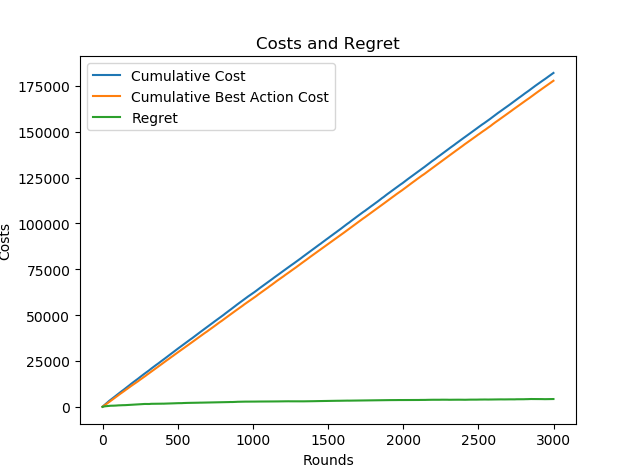
\includegraphics[width=3in]{spanning-cost-regret-uni.png}
        \end{minipage}
        \begin{minipage}[h]{0.5\linewidth}
            \centering
            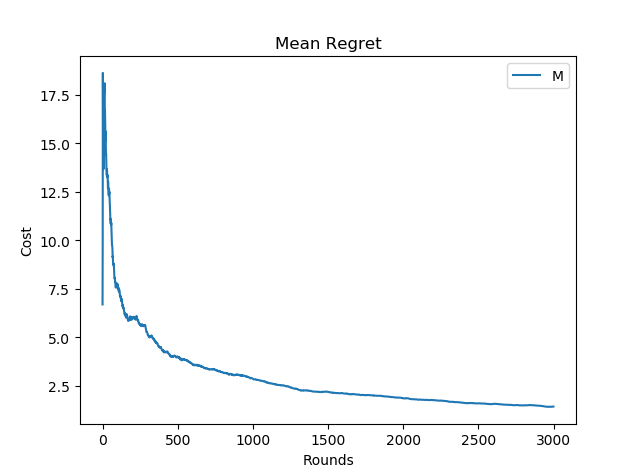
\includegraphics[width=3in]{spanning-mean-regret-uni.png}
        \end{minipage}
        \caption{The simulation result on a complete graph with 20 nodes. The weight of each edge is a uniform random variable with support $[m_i-3,m_i+3]$, where $m_i$ is chosen uniformly from $[3,5]$. The left figure shows the cost of the best action, our action, and the difference between them(regret). The right figure shows the average regret through time.}
        \label{spanning-uni}
    \end{figure}

    \begin{figure}[htbp!]
        \begin{minipage}[h]{0.5\linewidth}
            \centering
            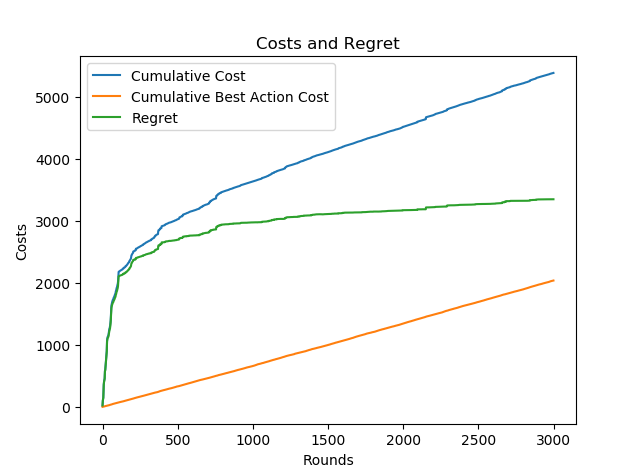
\includegraphics[width=3in]{spanning-cost-regret-weibull08.png}
        \end{minipage}
        \begin{minipage}[h]{0.5\linewidth}
            \centering
            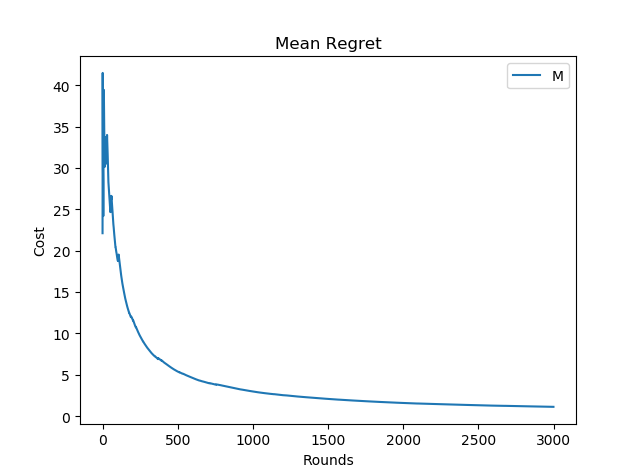
\includegraphics[width=3in]{spanning-mean-regret-weibull08.png}
        \end{minipage}
        \caption{The simulation result on a complete graph with 20 nodes. The weight of each edge is random variable $m_i \cdot x_i$, where $m_i,x_i$ are standard Weibull distrubution with parameter $0.8$. The left figure and the right figure shows the same things as in the previous figure.}
        \label{spanning-weibull08}
    \end{figure}

    \subsection{Minimize the Maximum Distance}
    \subsubsection{The case when the time is constant but unknown}

    We test the result of our method on a complete graph with 20 nodes. We test the situation when the weight random variable of each edge is a uniform random variable, and the results are shown in \textbf{Figure \ref{center-uni}}. We also simulate the case when the random variable of weight on each edge is $m_i\cdot x_i$ where $m_i,x_i$ are standard Weibull distribution with shape parameter $2$ and $0.7$, and the results are shown in \textbf{Figure \ref{center-weibull2},Figure \ref{center-weibull07}}.

    \begin{figure}[htbp!]
        \begin{minipage}[h]{0.5\linewidth}
            \centering
            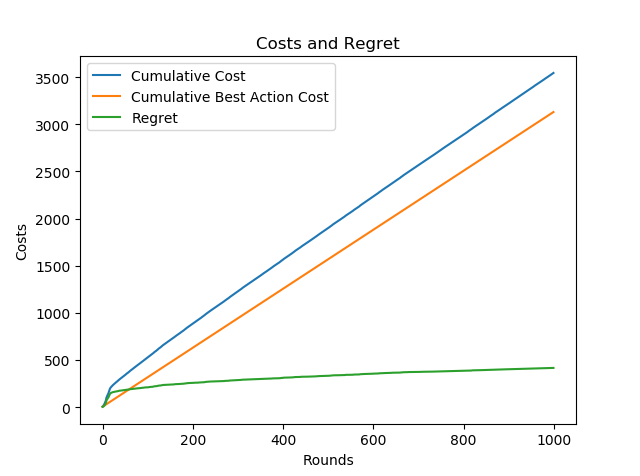
\includegraphics[width=3in]{simple-cost-regret-uni.png}
        \end{minipage}
        \begin{minipage}[h]{0.5\linewidth}
            \centering
            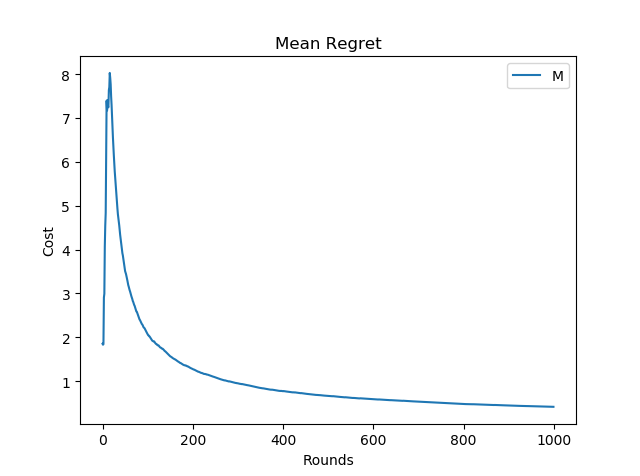
\includegraphics[width=3in]{simple-mean-regret-uni.png}
        \end{minipage}
        \caption{The simulation result on a complete graph with 20 nodes. The weight of each edge is a constant $m_i$, which is chosen uniformly from $[1,5]$. The left figure and the right figure shows the same things as in the previous figure.}
        \label{center-uni}
    \end{figure}

    \begin{figure}[htbp!]
        \begin{minipage}[h]{0.5\linewidth}
            \centering
            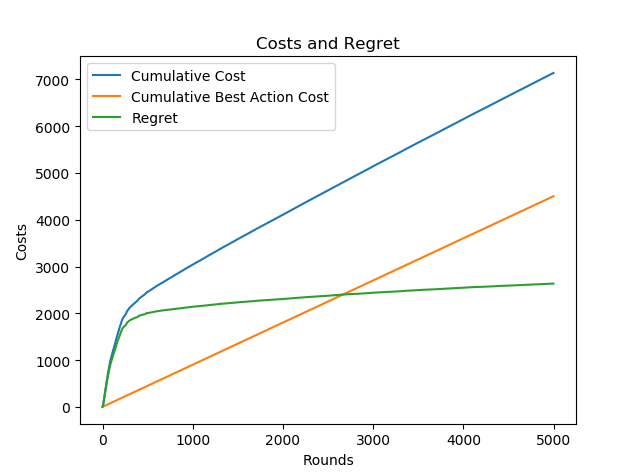
\includegraphics[width=3in]{simple-cost-regret-weibull2.png}
        \end{minipage}
        \begin{minipage}[h]{0.5\linewidth}
            \centering
            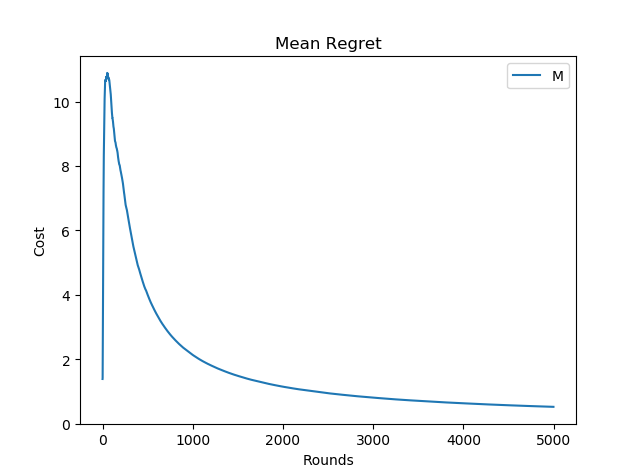
\includegraphics[width=3in]{simple-mean-regret-weibull2.png}
        \end{minipage}
        \caption{The simulation result on a complete graph with 20 nodes. The weight of each edge is random variable $m_i \cdot x_i$, where $m_i,x_i$ are standard Weibull distrubution with parameter $2$. The left figure and the right figure shows the same things as in the previous figure.}
        \label{center-weibull2}
    \end{figure}

    \begin{figure}[htbp!]
        \begin{minipage}[h]{0.5\linewidth}
            \centering
            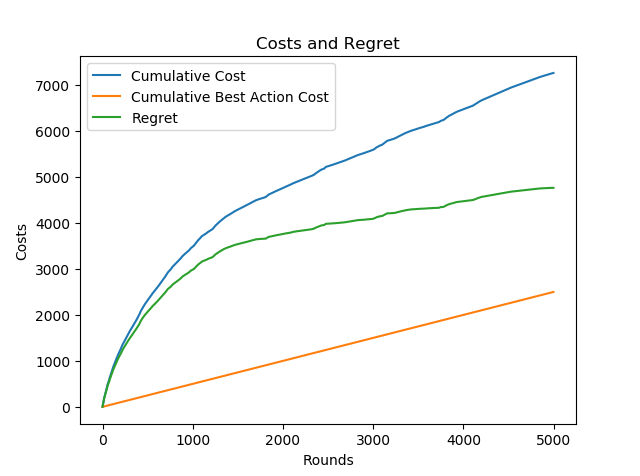
\includegraphics[width=3in]{simple-cost-regret-weibull07.png}
        \end{minipage}
        \begin{minipage}[h]{0.5\linewidth}
            \centering
            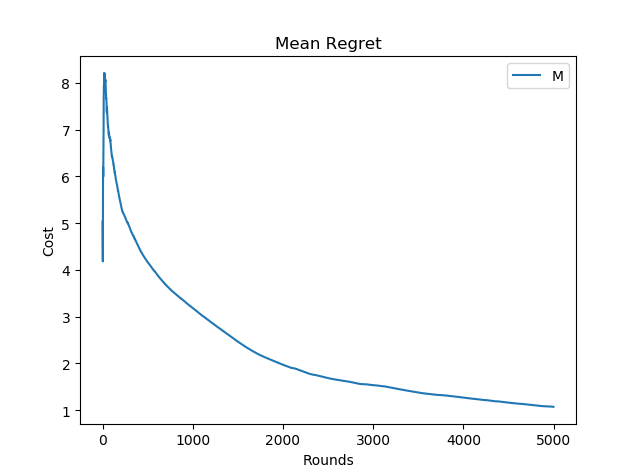
\includegraphics[width=3in]{simple-mean-regret-weibull07.png}
        \end{minipage}
        \caption{The simulation result on a complete graph with 20 nodes. The weight of each edge is random variable $m_i \cdot x_i$, where $m_i,x_i$ are standard Weibull distrubution with parameter $0.7$. The left figure and the right figure shows the same things as in the previous figure.}
        \label{center-weibull07}
    \end{figure}

    \subsubsection{The general case}

    We test our algorithm on the general case. Because our algoithm just find the best solution in the long term approximately, so it is not reasonble to test the difference between our action and the approximate solution. Here we test on the `cheated' best action, which knows the exact value of the random variables in each round and find the best solution on each round. The test results are shown in \textbf{Figure \ref{general-uni}}.

    \begin{figure}[htbp!]
        \begin{minipage}[h]{0.5\linewidth}
            \centering
            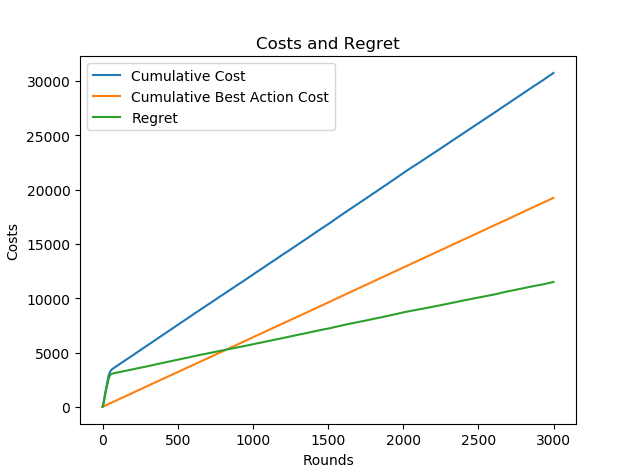
\includegraphics[width=3in]{general-cost-regret-uni.png}
        \end{minipage}
        \begin{minipage}[h]{0.5\linewidth}
            \centering
            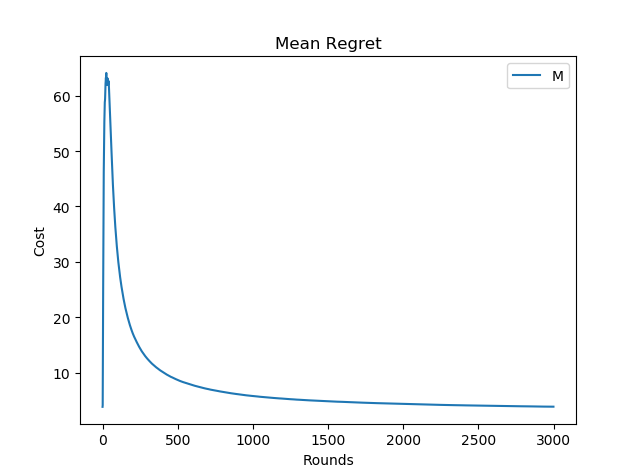
\includegraphics[width=3in]{general-mean-regret-uni.png}
        \end{minipage}
        \caption{The simulation result on a complete graph with 20 nodes. The weight of each edge is a uniform random variable with support $[m_i-3,m_i+3]$, where $m_i$ is chosen uniformly from $[4,8]$. The left figure shows the cost of the best action which `cheats' by find the best action each round, our action, and the difference between them. The right figure shows the average differnece through time.}
        \label{general-uni}
    \end{figure}

    \subsection{Analysis and Further Discussion}
    First from the simulation results, we find that the algorithm will converge almost to the best action except for the general case. We think that this is due to the fact that the previous cases only cares about the mean of each edge, which we try to approximate in our algorithm. But in the general case when the solution is not only based on the mean of each random variable but also the distribution of each random variable, our method may not converge to the best action.\\
    
    But the simulation results shows that our algorithm may also approximate the `cheating' solution to some constant, which may depend on the graph topology and the distribution of the random variable. Then combine our previous argument that when the information transfer through the shortest path tree rooted at the center, the time is at most $2$ times of the optimal strategy. So we can say that our strategy can solve this general case approximately.\\

    Moreover, we can find that the speed of convergence are differnet. When the distrubution has larger variance or the random variable is long tail, the speed of convergence is slow.

    \section{Conclusion}
    In this report, we study the online information synchronization problem, with known weight of the communication graph. We apply the framework in \cite{chen2013combinatorial} and let it fit our problem settings. We study the problem from $2$ different aspect, one from the minimum cost, and the other from the minimum time spent during the synchronization process. In the minimum cost version, we show that our method can tackle this problem successfully by simulation. However under the minimum time spent setting, our algorithm can successfully solve the problem when the random variables are constant and can only get a approximate solution of the general case.

    \newpage
    \bibliographystyle{ieeetr}
    \bibliography{mybib}

    
    \end{document}
    